\begin{figure}[t]
  \center
  \def\layersep{3cm}
  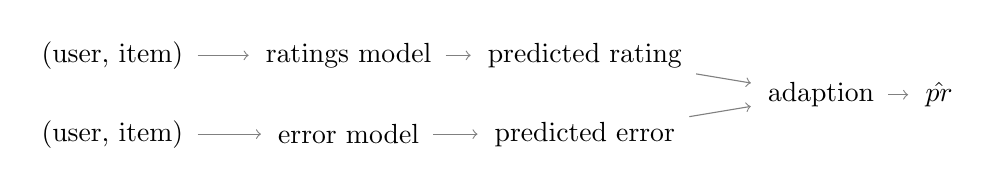
\begin{tikzpicture}[shorten >=1pt,->,draw=black!50, node distance=\layersep]

    \tikzstyle{every pin edge}=[<-,shorten <=2pt]
    \tikzstyle{rmodel}=[rectangle,fill=green!25,minimum size=20pt,inner sep=5pt]
    \tikzstyle{emodel}=[rectangle,fill=blue!25,minimum size=20pt,inner sep=5pt]
    \tikzstyle{amodel}=[rectangle,fill=red!25,minimum size=20pt,inner sep=5pt]
    \tikzstyle{blank}=[rectangle,fill=white,minimum size=20pt,inner sep=5pt]
    
    \node[blank] (UI1) at (0,-1) {(user, item)}; 
    \node[blank] (UI2) at (0,0) {(user, item)}; 

    \node[blank] (EM) at (\layersep,-1) {error model};
    \node[blank] (RM) at (\layersep,0) {ratings model};
    
    \node[blank] (ER) at (\layersep*2,-1) {predicted error};
    \node[blank] (RR) at (\layersep*2,0) {predicted rating};
 
    \node[blank] (AG) at (\layersep*3,-0.5) {adaption};
    \node[blank] (W) at (\layersep*3.5,-0.5) {$\hat{pr}$}; 
    
    \path (UI1) edge (EM);
    \path (UI2) edge (RM);
    \path (EM) edge (ER);
    \path (RM) edge (RR);
    \path (ER) edge (AG);
    \path (RR) edge (AG);
    \path (AG) edge (W);
       
  \end{tikzpicture}

  \vspace{1em}
  \caption[Adptive Weights]{
    Adaptive weights: The data flow through the adaption of a single recommender method.
    The current user and item is fed into two distinct models: the ratings model, which 
    predicts unknown ratings, and the error model, which predicts how accurate 
    this rating will be for the current input. 
    The two predictions are then aggregated into a final part of a rating ($\hat{pr}$).
    Each of the recommender stacks contribute parts to the final rating.
  }
  \label{fig:adaptiveweights}
\end{figure}
